\chapter{Optimización de ANGLE}\label{SecOptANGLE}
\begin{figure}
\centering
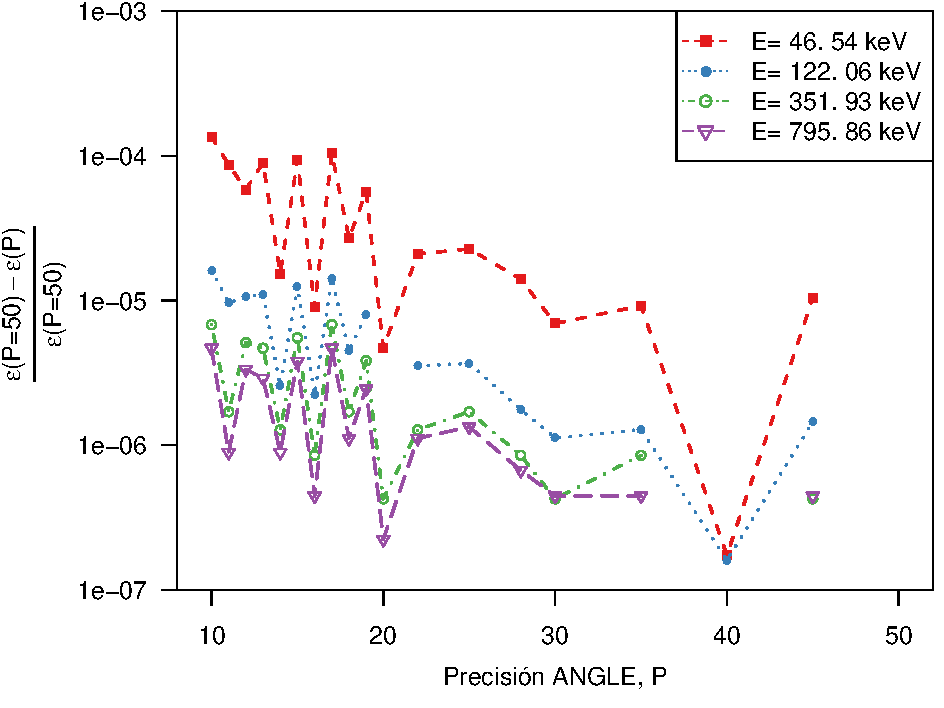
\includegraphics[width = \textwidth]{Imagenes/Eficiencia-precision-DiffPorcentual.pdf}
\caption{Gráfica de estabilidad de la eficiencia (ANGLE) para la sección 41 cm del núcleo GOMRI-500 y el sistema G2 en función de la precisión $P$ utilizada en relación a la precisión máxima, $P=50$.}\label{Fig-OptimizacionANGLE}
\end{figure}
\lettrine{E}{}l análisis de la precisión (parámetro $P$ de ANGLE) necesario para obtener los mejores resultados posibles con el mínimo esfuerzo de cómputo, se realizó utilizando la información de la sección 41 cm del núcleo GOMRI-500 con una composición desconocida del 50 \% de oxígeno. Para ello, se consideró la precisión máxima como la arrojada por el valor de $P$ máximo (50), y se calculó la diferencia respecto a este valor para diversos valores de $P$ (Figura \ref{Fig-OptimizacionANGLE}). Las diferencias observadas en todos los casos son muy pequeñas, lo que no justifica utilizar valores altos de $P$ alto. En base en el esfuerzo de cómputo requerido, se consideró adecuado utilizar un valor estándar de $P = 20$ para todos los análisis, excepto para los que requieren una simulación de Monte Carlo, para los que se utilizó el valor mínimo ($P=10$).